\documentclass{article}
\author{Jakob Graves}
\title{Graph Theory, Bondy, Murty \\ 1.1 Exercises}

\usepackage{amsmath}
\usepackage{graphicx}


\setlength{\parindent}{0pt}

\begin{document}
\maketitle

\section{Graphs and their representation}
\bigskip
\textbf{1.1.1 An upper bound on $\textit{\textbf{m}}$.}
\par\smallskip
Let $G$ be a simple graph. Show that $m \leq {n \choose 2}$, and determine when equality holds. 
\par\medskip Suppose for a contradiction that $m \geq {n \choose 2}$. In a simple graph, each edge is connected to two vertices, so there are ${n \choose 2}$ ways to connect $n$ vertices in a complete simple graph. So if $m \geq {n \choose 2}$, there must be a parallel edge or a loop. This implies that $G$ is not simple, a contradiction. 
\par Equality holds when the graph is complete, as noted above.

\bigskip\par\noindent\textbf{1.1.2 Bipartite upper bound on $\textit{\textbf{m}}$.} 
\par\smallskip
Let $G[X, Y]$ be a simple bipartite graph, where $|X|=r$ and $|Y|=s$.
\par\noindent (a) Show that $m\leq rs$
\par\noindent (b) Deduce that $m\leq n^2/4$
\par\noindent (c) Describe the simple bipartite graph for which equality holds in (b). 
\par\medskip\noindent
\textbf{(a)} In the complete bipartite graph, each vertex in $X$ is connected to all vertices in $Y$. So for each $x \in X$, there are $|Y|$ edges, each connecting to a $y \in Y$. Therefore, in the complete bipartite graph, there are $rs$ edges. Since the maximum number of edges occurs in the complete bipartite graph, we have $m\leq |X||Y|=rs$.
\par\noindent \textbf{(b)} In the case $r=s$, we have $r=s=n/2$. Then from (a), we see that $m\leq rs = (n/2)^2=n^2/4$. If $r<s$ (wlog), or if the graph is not complete, then $m<n^2/4$.
\par\noindent\textbf{(c)} Equality holds when the graph is complete and $r=s$.

\bigskip\par\noindent\textbf{1.1.3 Bipartite Graphs.}
\par\smallskip
Show that:
\par (a) every path is bipartite,
\par (b) a cycle is bipartite if and only if its length is even.
\par\smallskip
\textbf{(a)} The path can always be arranged as a bipartite graph, as in Figure 1, no matter the number of vertices.
\begin{figure}[h]
\centering
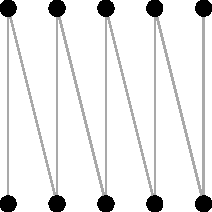
\includegraphics[width = 25mm]{1.1.3a.pdf}
\caption{\footnotesize{A 10-vertex bipartite path (needs to be cropped)}}
\end{figure}

This R code produced Figure 1 using the igraph package
\begin{quote}
\begin{verbatim}
	library(igraph)
	
	map <- unlist(bipartite_mapping(g)[2])
	
	plot(make_ring(n = 10, circular = FALSE),
	     layout = layout_as_bipartite(g, map),
	     vertex.color = "#000000",
	     vertex.label = NA)
\end{verbatim}
\end{quote}
We can confirm using igraph, first that the 10-cycle can be bipartite,
\begin{quote}
\begin{verbatim}
	bipartite_mapping(make_ring(n = 10, circular = TRUE))
	
	# $res
	# [1] TRUE
\end{verbatim}
\end{quote}
and that the 11-cycle cannot be bipartite.
\begin{quote}
\begin{verbatim}
	bipartite_mapping(make_ring(n = 11, circular = TRUE))
	
	# $res
	# [1] FALSE
\end{verbatim}
\end{quote}

\bigskip\par\textbf{1.1.4 Average vertex degrees.}
\par\smallskip
Show that, for any graph $G$, we have $\delta(G) \leq d(G) \leq \Delta(G)$, where $\delta(G)$ is the minimum vertex degree, $d(G)$ is the avergae vertex degree, and $\Delta(G)$ is the maximum vertex degree.
\par\smallskip
Consider the vertex degrees in ascending order: $\{\delta G, d(v_2), \ldots , d(v_{n-1}), \Delta (v_n)\}$, and consider the related set $\{\delta (G) - \delta (G), d(v_2) - \delta (G), \ldots , \Delta (G) - \delta (G)\}$. The mean of the second set is simply the mean of the first set minus the minimum degree. The numbers in the second set must all be greater than or equal to 0 by definition of the minimum, so the mean must be greater than or equal to 0. Therefore, the minimum vertex degree must always be less than or equal to the mean. 
\par Alternatively, for the second part, consider the same list of vertices in ascending order: $\{\delta (G) - \delta (G), d(v_2) - \delta (G), \ldots , \Delta (G) - \delta (G)\}$. Then the average is $$\frac{\sum_i d(v_i)}{n} = d(G)$$ Therefore, $$nd(G)=\sum_i d(v_i) \leq n\Delta(G)$$ Finally, we have $nd(G)\leq n\Delta(G)$ and so $d(G) \leq \Delta(G)$, and the mean is less than the maximum.
 
\bigskip\par\textbf{1.1.5 $\textit{\textbf{k}}$-regular graphs.}
\par\smallskip
For $k = 0, 1, 2$, characterize the $k$-regular graphs. 
\begin{itemize}
\item With $k =0$, the set can be characterized as all graphs consisting of only disconnected vertices.
\item With $k=1$, the set can be characterized as all graphs consisting of only disconnected edges.
\item With $k=2$, the $k$-regular graphs are all cycles and all infinite paths.
\end{itemize}

\bigskip\par\textbf{1.1.6 Vertex symmetries.}
\par\smallskip
(a) Show that, in any group of two or more people, there are always two who have exactly the same number of friends.\par
(b) Describe a group of five people, any two of whom have exactly one friend in common. Can you find a group of four people with the same property?
\par\smallskip\textbf{(a)} Let us represent the individuals as vertices, and friendships as edges. Clearly, this graph is simple. If there are $n$ people in the group, then the possible number of friends for each person is $\{0, 1, 2, 3, \ldots, n-1 \}$. So if no two people have the same number of friends, then the degree sequence is $\{0, 1, 2, \ldots, n-1\}$. But this simple graph is not possible, since if one vertex has degree 0, then it must have no adjacent edges. Therefore, the maximum degree of the remaining vertices is $n-2$.
\par\textbf{(b)} The group of five is shown as a graph below. The code to generate this graph is also below. 
\begin{figure}[h]
\centering
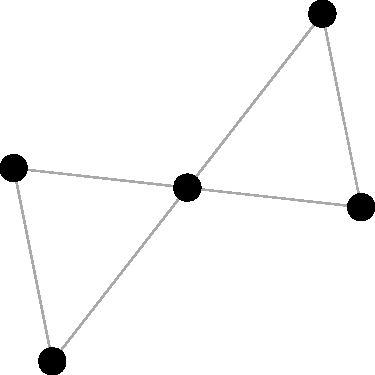
\includegraphics[width = 30mm]{1.1.6b.pdf}
\caption{\footnotesize{A group of five people, any two of whom have exactly one friend in common}}
\end{figure}
\begin{quote}
\begin{verbatim}
	library(igraph)
	adjmat.data <- c(0,1,1,1,1,
	                 1,0,0,1,0,
	                 1,0,0,0,1,
	                 1,1,0,0,0,
	                 1,0,1,0,0)
	mat <- matrix(adjmat.data, nrow=5, ncol=5, byrow=TRUE)
	
	plot(graph_from_adjacency_matrix(mat, mode="undirected"),
		     vertex.color = "#000000", 
	     vertex.label = NA)
\end{verbatim}
\end{quote}


\bigskip\par\textbf{1.1.7 $\textit{\textbf{n}}$-cube}
\par\smallskip
The $n-cube$ $Q_n$ $(n \geq 1)$ is the graph whose vertex set is the set of all $n$-tuples of 0s and 1s, where two $n$-tuples are adjacent if they differ in precisely one coordinate. 
\par\smallskip
(a) Draw $Q_1, Q_2, Q_3,$ and $Q_4$.
\par
(b) Determine $v(Q_n)$ $e(Q_n)$.
\par
(c) Show that $Q_n$ is bipartite for all $n \geq 1$.
\par\smallskip\textbf{(a)}
\begin{figure}[ht]
\centering
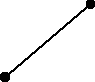
\includegraphics[width = 25mm]{1.1.7ai.pdf}
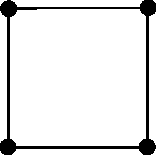
\includegraphics[width = 25mm]{1.1.7aii.pdf}
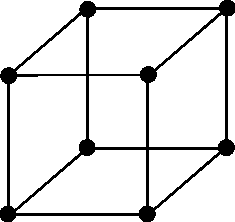
\includegraphics[width = 25mm]{1.1.7aiii.pdf}
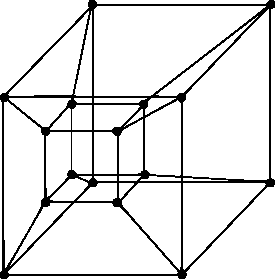
\includegraphics[width = 25mm]{1.1.7aiv.pdf}
\end{figure}
\par\smallskip\textbf{(b)} Clearly, the number of different $n$-tuples of 1s and 0s for a given $n$ is equal to $$v(Q_n)=2^n$$ For the edges, we note that the $n$-cube (remember $n$ is the degree of each vertex) is a $n$-regular graph. The number of edges in a $n$ regular graph is $Nn/2$ where $N$ is the order of the graph, so $N=v(Q_n)$. So we have that $$e(Q_n)=n2^{n-1}$$
\par\smallskip\textbf{(c)} 


\bigskip\par\textbf{1.1.9 Vertex degrees in bipartite graphs.}
\par\smallskip
Let $G[X,Y]$ be a bipartite graph.
\par\smallskip
(a) Show that $\sum_{v\in X}d(v)=\sum_{v\in Y}d(v)$
\par
(b) Deduce that if $G$ is $k$-regular, with $k \geq 1$, then $|X|=|Y|$.
\par\smallskip
\textbf{(a)} Consider the bipartite adjacendy matrix. It looks something like this:
\[A= \left[ 
\begin{array}{cc | ccc}
    0 & 0 &  a_{1,3}  & \cdots & a_{1,n} \\
     0 & 0 & a_{2,3}  & \cdots & a_{2,n} \\
 \hline
     a_{3,1} & a_{3,2} & 0  & \cdots & 0 \\
      \vdots & \vdots & \vdots  & \ddots & \vdots \\
     a_{n,1} & a_{n,2} & 0  & \cdots & 0 \\
\end{array} \right]
\]
Let the partitions above the horizontal line be part of $X$ and the partitions below the horizontal line $Y$.
\par\medskip
The row sum is the number of edges connected to the respective vertex (each row corresponds to a vertex in the adjascency matrix). The sum of row $i$ is therefore $d(v_i)$. Similarly, the sum of column $j$ is $d(v_j)$.
\par\medskip
The form of the adjacency matrix for a general bipartite graph is 
\[ A=
\begin{bmatrix}
0 & B\\
B^T & 0\\
\end{bmatrix}
\]
since each edge has an endpoint in both $X$ and $Y$. So it follows that
$$\sum_{v\in V}d(v)=2\sum_{b\in B}b=2\sum_{b\in B^T}b$$
Then since the elements in $B$ are the same as those in the partition that corresponds to $X$ (and the elements in $B^T$ are the same as those that correspond to the $Y$ partition), and recalling that the sum of elements in row (column) $i$ is equal to $d(v_i)$, we have
$$2\sum_{b\in B}b=2\sum_{v\in X}d(v)=2\sum_{v\in Y}d(v)=2\sum_{b\in B^T}b$$
which is equivalent to the desired result 
$$\sum_{v\in X}d(v)=\sum_{v\in Y}d(v)$$









\end{document}

